\documentclass[12pt,a4paper]{article}
\usepackage[utf8]{inputenc}
\usepackage{graphicx}
\usepackage{float}
\usepackage{subcaption}
\usepackage[margin=1in]{geometry}
\usepackage{hyperref}
\usepackage{url}
\hypersetup{
  pdfborder = {0 0 0}
}
\usepackage[
backend=biber,
style=alphabetic,
]{biblatex}

\addbibresource{NAK.bib}

\graphicspath{{./NAK/}}
\DeclareGraphicsExtensions{.pdf,.jpeg,.jpg,.png}

\usepackage{amsmath} % equations
\usepackage{fancyhdr} % nicer page header

\setlength{\parindent}{0pt} % no paragraph indents
\setlength{\parskip}{1em} % paragraphs separated by one line

\newcommand\experiment{Neutron Activation} %% experiment name
\newcommand\groupno{Group 3}       %%%%% group number
\newcommand\names{Pratyush Singh,\\
                  Proshmit Dasputpa\\}        %%%%% full names
\newcommand\expdate{21/03/2025}    %%%%% date of experiment day

\begin{document}
\begin{titlepage}
   \begin{center}
        \vspace*{3cm}
        \Huge{\experiment}
				
        \vspace{0.5cm}
        \LARGE{Lab course protocol}
				
        \vspace{3 cm}
        \Large{\groupno}
				
        \vspace{0.25cm}
        \large{\names}
				
        \vspace{2 cm}
        \Large{\expdate}
				
        \vspace{0.25 cm}
        \Large{Advanced lab course in astronomy\\
				Eberhard Karls Universit\"at T\"ubingen}
				
				\vspace{0.1 cm}
        \Large{WiSe 2024/25}
				
       \vfill
    \end{center}
\end{titlepage}

\pagestyle{fancy}
\fancyhf{}
\setlength{\headheight}{14.5pt}
\lhead{\groupno; \experiment}

%\section*{Abstract}
% This is optional, but never longer than half a page.

\tableofcontents
\newpage

\setcounter{page}{1}
\pagestyle{fancy}
\fancyhf{}
\rhead{\thepage}
\lhead{\groupno; \experiment}

\section{Introduction}

In this experiment, natural samples of silver and indium are activated using slow (thermal) neutrons from an AmBe (Americium-Beryllium) source. This process, known as \textit{\textbf{neutron activation}}, results in the formation of radioactive isotopes through neutron capture. \\ The decay of these isotopes is tracked using Geiger-Müller counters, enabling the determination of their \textbf{decay curves}, \textbf{half-lives}, and \textbf{initial activities}. This technique, called \textit{\textbf{Neutron Activation Analysis (NAA)}} - is a powerful, non-destructive method widely used in material analysis and nuclear research.

\section{Theory}

\subsection{Radioactivity: $\alpha$, $\beta$, and $\gamma$ Decay}

Radioactive decay is the spontaneous transformation of an unstable atomic nucleus into a more stable one, accompanied by the emission of particles or electromagnetic radiation:

\begin{itemize}
  \item \textbf{$\alpha$-decay}: Emission of a helium nucleus ($^4_2\mathrm{He}$), typical for heavy nuclei with a proton surplus. It has a short range (usually only a few \textit{centimetres} in air) and is easily shielded.
  \item \textbf{$\beta$-decay}: These type of decays are a result of the weak interaction (weak nuclear force). $\beta$-decays have two subtypes:
    \begin{itemize}
      \item \textbf{$\beta^-$}: A neutron transforms into a proton, emitting an electron and an antineutrino: 
      \[
      n \rightarrow p + e^- + \bar{\nu}_e
      \]
      \item \textbf{$\beta^+$}: A proton becomes a neutron, emitting a positron and a neutrino:
      \[
      p \rightarrow n + e^+ + \nu_e
      \]
    \end{itemize}
  \item \textbf{$\gamma$-emission}: The nucleus transitions from an excited to a lower energy state, emitting a high-energy photon:
  \[
  ^A_ZX^* \rightarrow ^A_ZX + \gamma
  \]
  Most of the time, these high energy photons interact with matter in three ways - \textit{photo effect}, \textit{Compton effect} and \textit{pair production}.
\end{itemize}

\subsection{Activity}

The \textit{activity} $A(t)$ of a radioactive sample is the number of decays per unit time:
\[
A(t) = \lambda N(t) = \lambda N_0 e^{-\lambda t}
\]
where:
\begin{itemize}
  \item $\lambda$ is the decay constant,
  \item $N(t)$ is the number of undecayed nuclei at time $t$, and $N_0$ is the initial number of nuclei.
  \item $A$ is measured in \textbf{Becquerel (Bq)}, where $1~\mathrm{Bq} = 1~\mathrm{decay/s}$.
\end{itemize}

The \textit{half-life} $t_{1/2}$ (i.e, the time after which exactly \textit{half} of the initial activity remains) is given by:
\[
t_{1/2} = \frac{\ln 2}{\lambda}
\]

\subsection{Differential Equations for Decay and Activation}

For pure radioactive decay without any kind of external input:
\[
\frac{dN}{dt} = -\lambda N
\]

When new radioactive nuclei are being produced (e.g., during activation), the equation becomes:
\[
\frac{dN}{dt} = -\lambda N + P
\]
where $P$ is the \textbf{production rate}. Solving this gives the time-dependent activity:
\[
A(t_a) = A_S \left(1 - e^{-\lambda t_a}\right)
\]
with $A_S = \sigma \Phi n$ as the \textbf{saturation activity}, and $t_a$ being the \textbf{activation time}.

\subsection{Saturation Activity}

The \textit{saturation activity} $A_S$ is the maximum activity that can be reached under continuous irradiation:
\[
A_S = \sigma \Phi n
\]
It is approached asymptotically as $t_a \rightarrow \infty$. This value depends on:
\begin{itemize}
  \item $\sigma$: Neutron capture cross-section,
  \item $\Phi$: Neutron flux,
  \item $n$: Number of target atoms in the irradiated sample.
\end{itemize}

\subsection{Creation of Free Neutrons}

Free neutrons are not stable in nature (mean lifetime $\sim$ 886 s) and must be produced via nuclear reactions. In this experiment, a \textbf{($\alpha$, n)} reaction in an AmBe source is used:

\[
^9\mathrm{Be} + \alpha \rightarrow ^{12}\mathrm{C} + n
\]

Here, $^{241}$Am emits $\alpha$ particles, which interact with $^9$Be to release neutrons. The resulting fast neutrons are slowed down (moderated) using paraffin to become \textit{thermal neutrons} ($E \approx 0.025~\mathrm{eV}$), which are highly effective in neutron capture reactions.

An example of neutron capture (an $(n,\gamma)$ reaction) relevant to this experiment:
\[
\mathrm{Ag}^{107,109} + n \rightarrow \mathrm{Ag}^{108,110*} \rightarrow \mathrm{Ag}^{108,110} + \gamma
\]

These reactions result in radioactive isotopes whose decay can then be studied.







\section{Experiments}

\subsection{Description of the Experimental Procedure}

The experiment is divided into several parts, starting with detector calibration and background measurement, followed by the activation and decay analysis of silver and indium samples. The following steps summarize the procedure:

\begin{enumerate}
  \item \textbf{Calibration of the Geiger-Müller counters:}
  \begin{itemize}
    \item A \textsuperscript{60}Co source is placed next to the detector for calibration.
    \item The voltage applied to the GM tubes is varied incrementally, and the corresponding count rates are recorded using a scaler.
    \item A voltage vs. count rate plot is created to identify the plateau region.
    \item The working voltage is chosen within the first third of the plateau to ensure stable operation.
  \end{itemize}

  \item \textbf{Measurement of the background radiation:}
  \begin{itemize}
    \item With no active source or sample present, a 60-minute background measurement is taken. We have taken a 45-minute measurement.
    \item Data is recorded in intervals of $\Delta t = 60$ s using the \texttt{Cassylab} software. For our experiment, we have used a $5$ minute interval.
  \end{itemize}

  \item \textbf{Preparation of the samples:}
  \begin{itemize}
    \item Natural silver and indium metal samples are used.
    \item Samples are handled only with pliers and inserted into the neutron source using aluminum rods.
    \item Care is taken to avoid contact with the rod ends that are inserted into the source, due to their own activation.
  \end{itemize}

  \item \textbf{Activating and measuring the decay of silver:}
  \begin{itemize}
    \item The silver sample is irradiated for various activation times: 5 s, 10 s, 20 s, 30 s, 45 s, 60 s, 90 s, 2 min, 5 min, and 15 min.
    \item After irradiation, the sample is quickly transferred to the detector setup.
    \item Decay measurements are conducted for 400 s total duration, with a counting interval of $\Delta t = 5$ s.
    \item The time offset between the end of irradiation and start of measurement is recorded with a stopwatch for later correction.
  \end{itemize}

  \item \textbf{Activating and measuring the decay of indium:}
  \begin{itemize}
    \item The indium sample is irradiated and then measured in the same manner as the silver sample.
    \item Decay is recorded using the parameters: 30 minutes total, with $\Delta t = 5$ s intervals.
    \item The activation time and timing offset are recorded.
  \end{itemize}
\end{enumerate}

\subsection{Sketch and Description of the Neutron Source}

The neutron source used is a moderated Americium-Beryllium (AmBe) source embedded within a layered shielding structure:

\begin{itemize}
  \item The source emits $\alpha$ particles from \textsuperscript{241}Am, which interact with beryllium to release neutrons via the $(\alpha,n)$ reaction.
  \item It is housed inside a cube of paraffin (edge length: 150 cm), with inner solid paraffin and outer layers made of borated paraffin bricks.
  \item A 1 cm thick lead shield surrounds the source to block $\gamma$ radiation.
  \item The sample holder is inserted into slits at the back of the assembly, which have direct line-of-sight to the neutron source.
\end{itemize}

\begin{figure}[H]
  \centering
  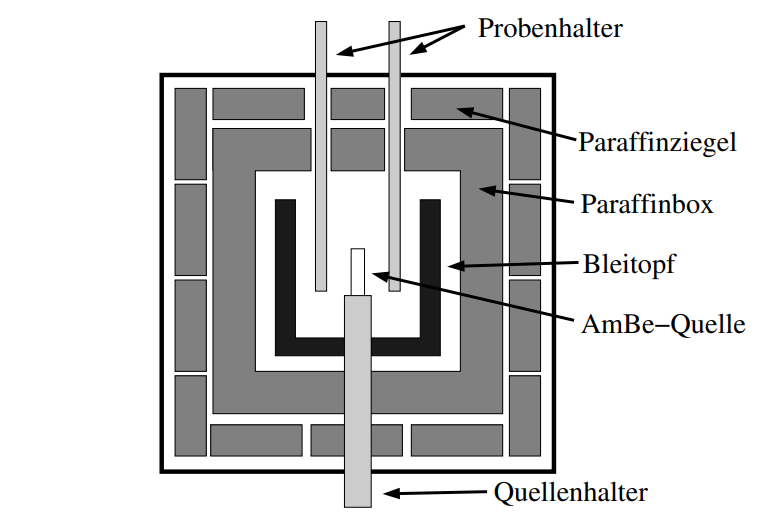
\includegraphics[width=0.7\textwidth]{Pictures/AmBe Source.png}
  \caption{AmBe source setup (Schematic).}
  \label{fig:AmBe}
\end{figure}

\subsection{Sketch and Working Principle of the Detector}

In this experiment, a Geiger-Müller (GM) counter is used to detect the radiation emitted by the activated silver and indium samples. The GM counter is a type of gaseous ionization detector, consisting of a cylindrical tube filled with a noble gas at low pressure and a central wire anode. When ionizing radiation enters the detector through a thin mica window, it ionizes the gas, creating electron-ion pairs.

Due to the high voltage applied across the electrodes, these primary electrons are rapidly accelerated, gaining enough energy to cause further ionization — resulting in an \textit{avalanche} of secondary electrons. This avalanche produces a measurable current pulse, which is counted as a detection event.

In the \textit{Geiger-Müller (plateau) region}, the size of the output pulse is independent of the energy of the incoming radiation, allowing only particle counting, not energy discrimination. To prevent continuous discharge, the tube includes a \textit{quenching gas} that limits the avalanche.

While GM counters cannot differentiate between types or energies of radiation, they are extremely useful for measuring decay rates and background radiation due to their simplicity and sensitivity.

In this experiment, two GM tubes are used, and the operating voltage is chosen from the plateau region of the tube's characteristic curve, ensuring a stable response.

\begin{figure}[H]
  \centering
  \begin{subfigure}{0.49\textwidth}
    \centering
    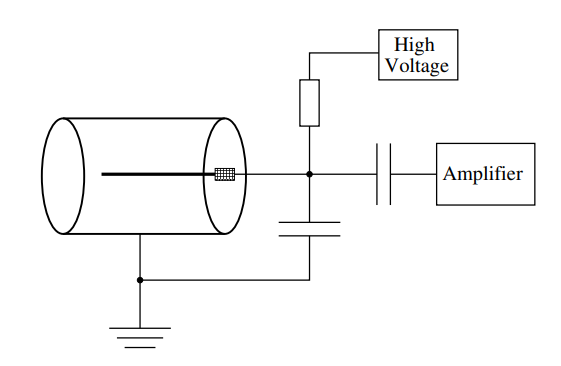
\includegraphics[width=1.0\textwidth]{Pictures/GM_Schematic.png}
    \caption{Working principle of a Geiger-Müller counter}
    \label{fig:GM_schematic}  
  \end{subfigure}
  \begin{subfigure}{0.49\textwidth}
    \centering
    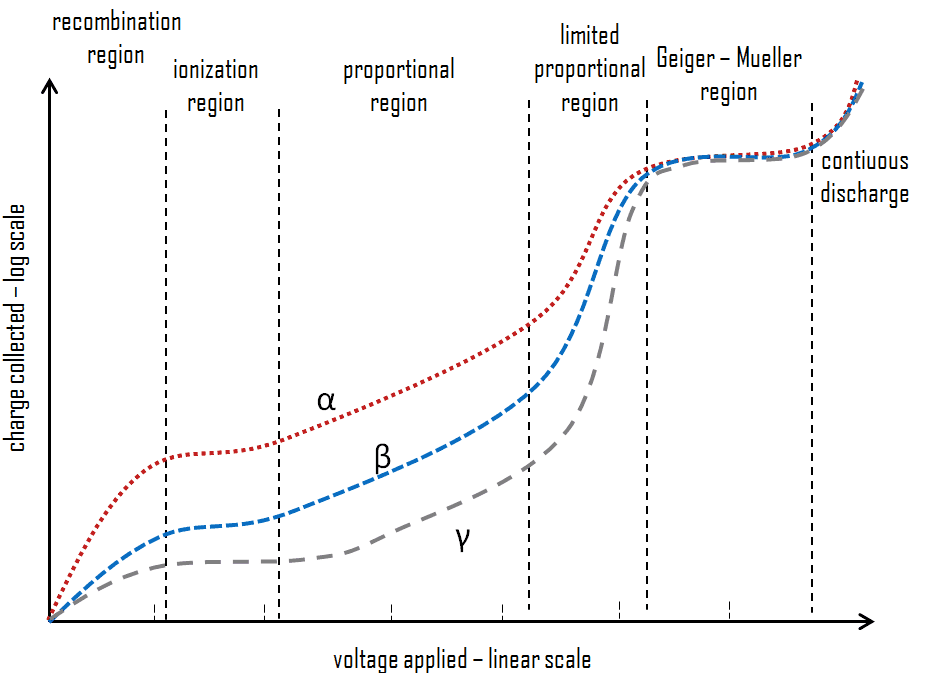
\includegraphics[width=1.0\textwidth]{Pictures/GM_IV.png}
    \caption{I-V characteristic curve of a GM counting tube (Source: \cite{GM})}
    \label{fig:GM_IV}
  \end{subfigure}
  \caption{Schematic diagram of a Geiger-Müller counter and its I-V characteristic curve. The plateau region is used in this experiment for stable operation.}
\end{figure}

\subsection{Capture and Decay Reactions of Relevant Isotopes}

\begin{itemize}
  \item \textbf{Silver Activation (natural silver contains \textsuperscript{107}Ag and \textsuperscript{109}Ag):}
  \[
  ^{107}\mathrm{Ag} + n \rightarrow ^{108}\mathrm{Ag}^* \rightarrow ^{108}\mathrm{Ag} + \gamma \quad (\text{T}_{1/2} \approx 2.4 \, \text{min})
  \]
  \[
  ^{109}\mathrm{Ag} + n \rightarrow ^{110}\mathrm{Ag}^* \rightarrow ^{110}\mathrm{Ag} + \gamma \quad (\text{T}_{1/2} \approx 24 \, \text{s})
  \]

  \item \textbf{Indium Activation (natural indium is mostly \textsuperscript{115}In):}
  \[
  ^{115}\mathrm{In} + n \rightarrow ^{116}\mathrm{In}^* \rightarrow ^{116}\mathrm{In} + \gamma \quad (\text{T}_{1/2} \approx 54 \, \text{min})
  \]

  \item These reactions produce radioactive isotopes that decay via $\beta^-$ emission, and their decay rates are measured in this experiment.
\end{itemize}
\subsubsection*{Branching Ratios}

In general, radioactive isotopes can decay via multiple channels, each with a characteristic probability known as the \textit{branching ratio}. These ratios quantify the likelihood of a nucleus decaying through a particular path relative to all possible decay modes. 

In this experiment, however, the activation products (\textsuperscript{108}Ag, \textsuperscript{110}Ag, and \textsuperscript{116}In) \textbf{decay predominantly via a single $\beta^-$ decay mode}. As a result, only the main decay channel is considered in the analysis, and branching ratios are not treated separately in the data evaluation. Nevertheless, they are implicitly reflected in the total measured activity.

\section{Analysis}
\subsection{Plateau Curve and Operating Voltage}

To determine a suitable operating voltage for the Geiger-Müller counters, the count rate was measured as a function of applied voltage using a \textsuperscript{60}Co calibration source. The resulting plateau curves for both the left and right detectors are shown in Figure. (Add reference) 

The plateau region corresponds to the range where the count rate remains approximately constant despite increasing voltage, indicating stable detector operation. Based on the curves, a voltage of 325 V was selected, lying within the first third of the plateau. This ensures reliable detection while minimizing the risk of continuous discharge or excessive dead time.




\setcounter{secnumdepth}{0}

\printbibliography
\appendix
\section{Appendix}




\end{document}